\documentclass[../Analysis-3.tex]{subfiles}

\begin{document}
\chapter*{Lecture 21} %Set chapter name
\addcontentsline{toc}{chapter}{Lecture 21} %Set chapter title
\setcounter{chapter}{21} %Set chapter counter
\setcounter{section}{0}

\section{Change of Variables (Continued)}

\begin{Thm}{Change of Variables}{21:1}
  Let $\mathcal{O}_n \subseteq \R^n$ be open, and $\varphi : \mathcal{O}_n \to \R^n$ be a $C^1 $ and injective function, and $\det ( J_{\varphi}(x) ) \neq 0$ for all $x \in \mathcal{O}_n$. Let $\Omega \subseteq \mathcal{O}_n$ such that $\Omega \cup \partial \Omega \subseteq \mathcal{O}_n$ and $\partial \Omega$ is of content zero. If $f \in \mathscr{R}(\varphi(\Omega))$, then
  \[
    \int_{\varphi(\Omega)} f = \int_{\Omega} (f \circ \varphi) |\det J_{\varphi}|
  \]
\end{Thm}

Now let's look at some examples of change of variables.

\begin{Eg}{Polar Co-ordinates}{}
  \begin{wrapfigure}{r}{0.45\textwidth}
    \centering
    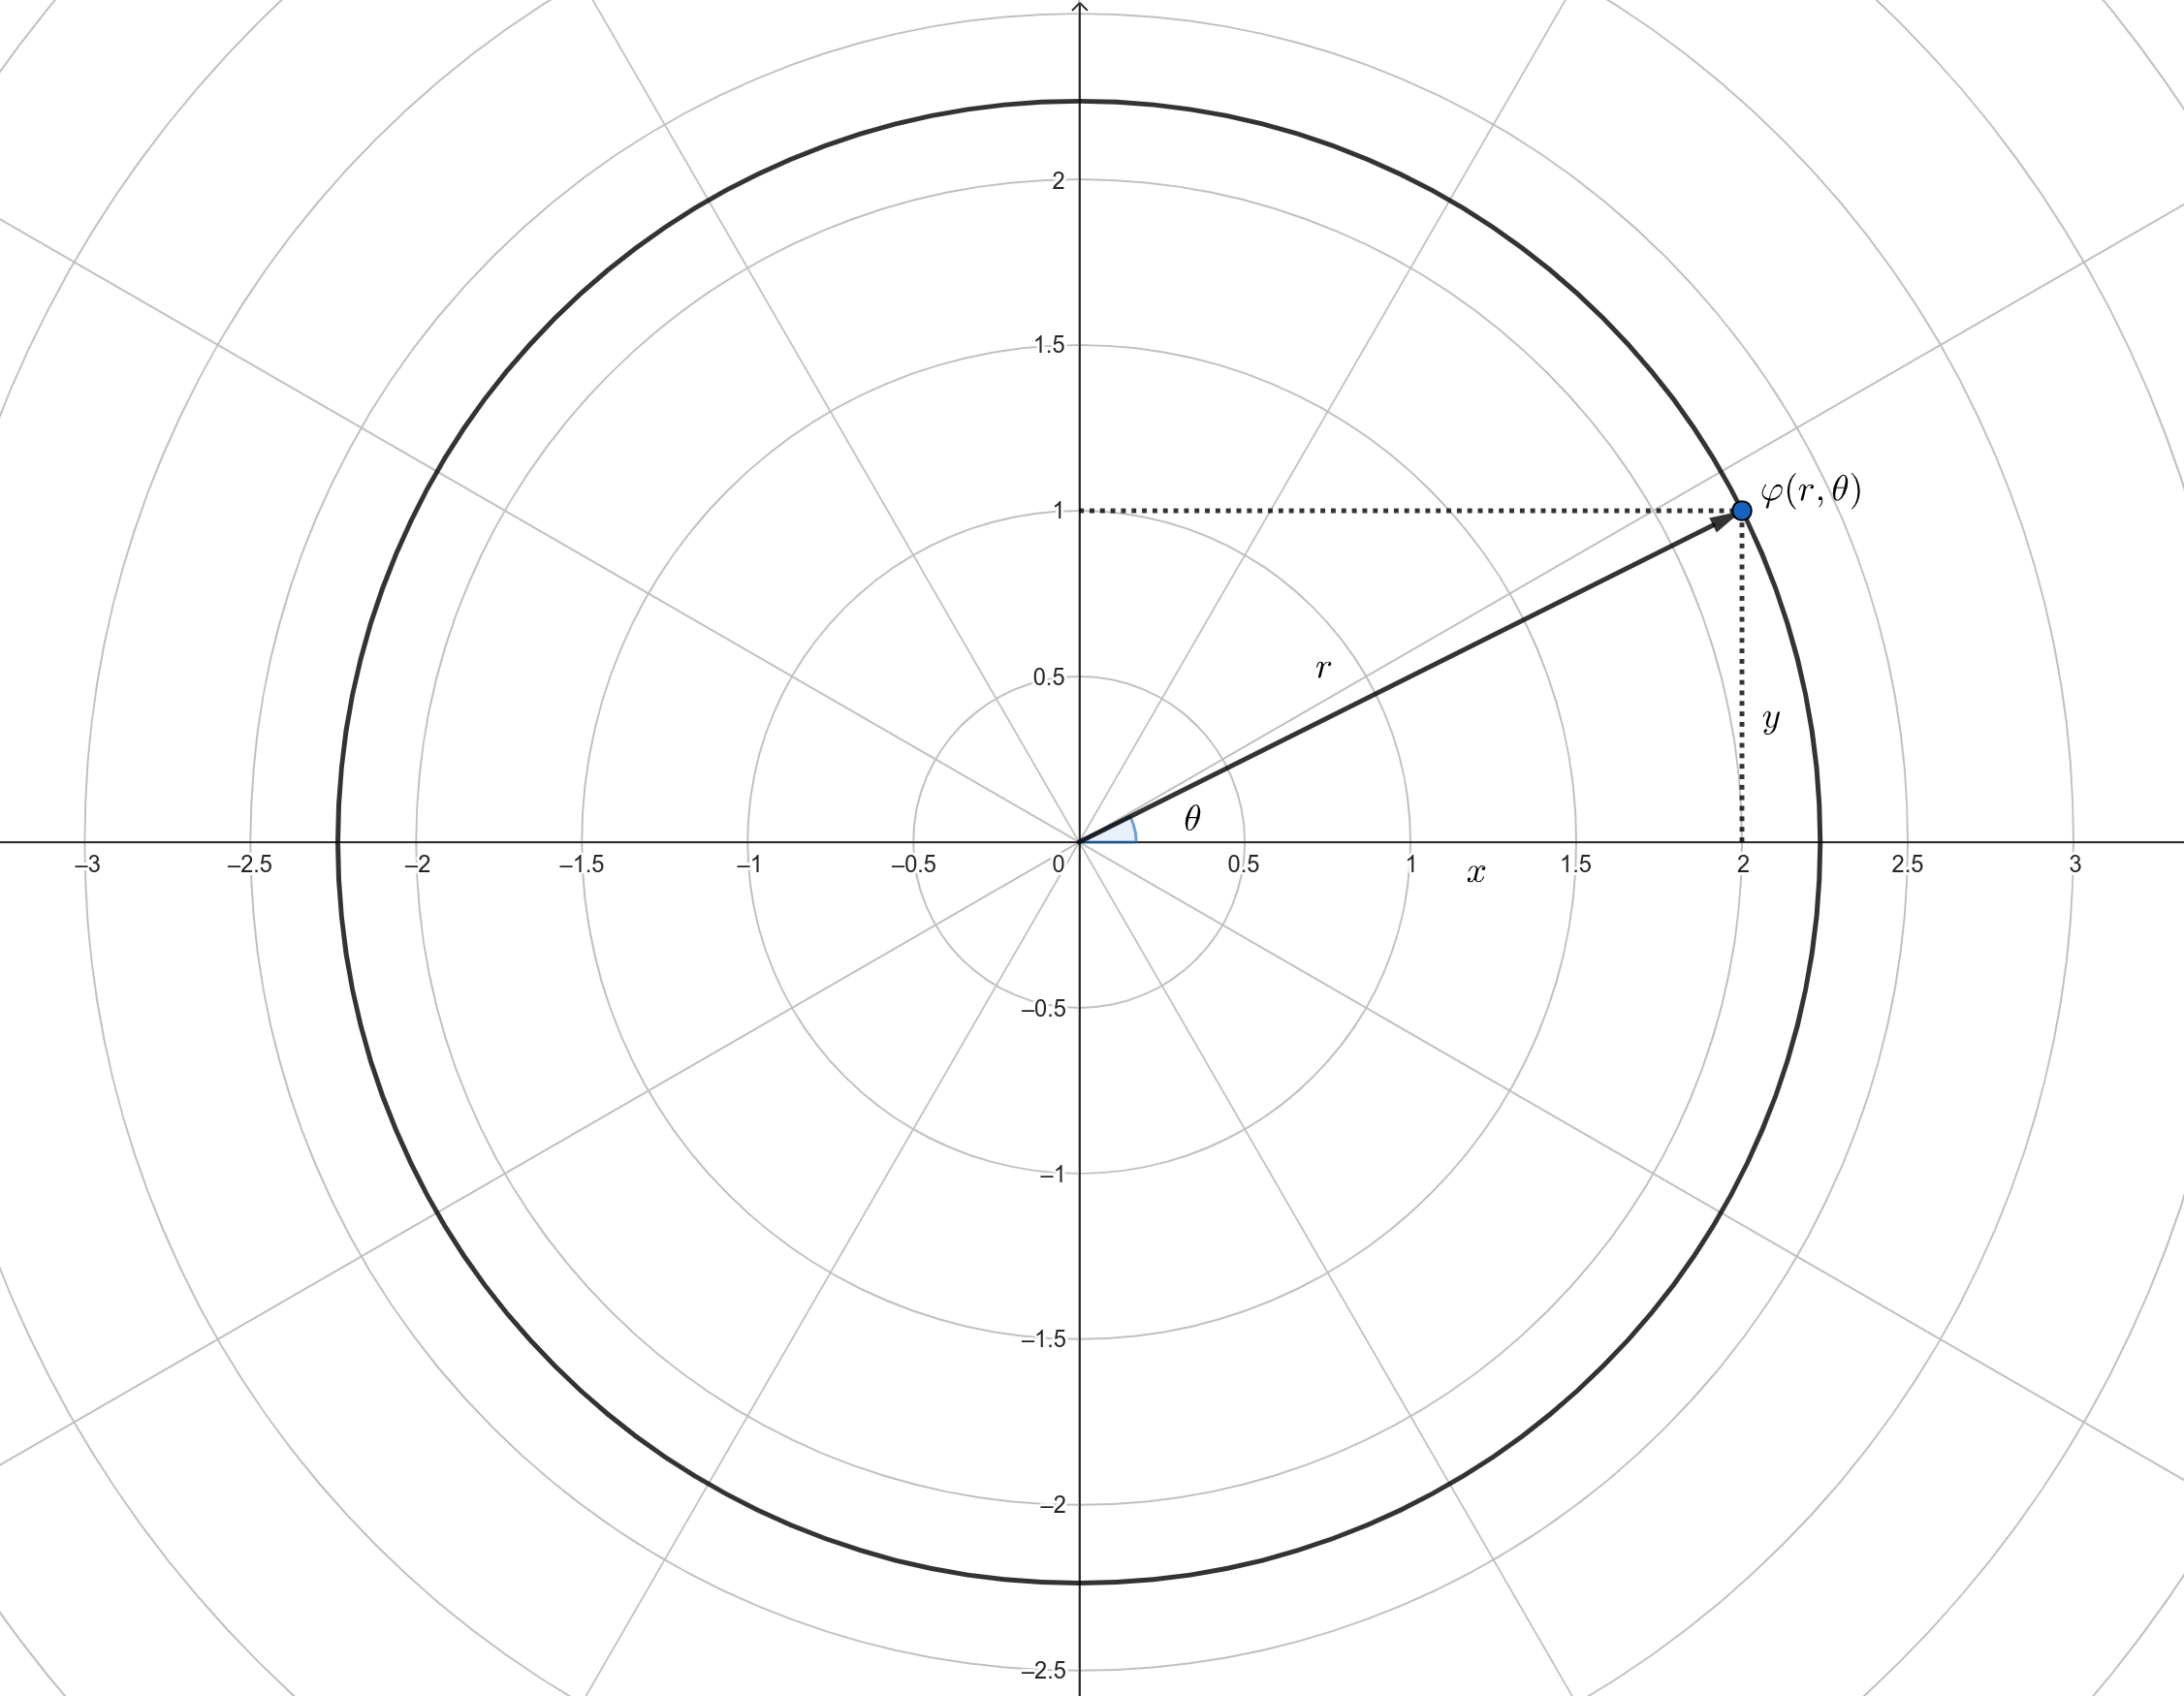
\includegraphics[width=0.5\textwidth]{../figures/lec21.1.png}
    \caption{Transforming into polar coordinates}
    \label{fig1:21}
  \end{wrapfigure}
  While solving some problems, it's sometimes better to work with polar coordinates than to use Cartesian coordinates, this example illustrates how we can go to polar coordinates from Cartesian coordinates.
  Consider $\varphi : \R^2 \to \R^2$ as follows $\varphi(r,\theta) = (r \cos\theta, r \sin\theta)$. Then Jacobian of $\varphi$ is given by
  \[
    J_{\varphi}(r,\theta) = \begin{bmatrix}
      \cos\theta & -r\sin\theta \\
      \sin\theta & r\cos\theta
    \end{bmatrix} \Rightarrow \det(J_{\varphi}(r,\theta)) = r
  \]
  Thus $\det(J_{\varphi}(r,\theta)) \neq 0 \Leftrightarrow r \neq 0$. So consider $\mathcal{O}_2 := (0,\infty) \times (0,2\pi)$. Then $\varphi\vert_{\mathcal{O}_2} : \mathcal{O}_2 \to \R^2$ is $C^1$ and injective function and $\det(J_{\varphi}(r,\theta)) \neq 0 $ on $\mathcal{O}_2$. Now given $0 < r_1 < r_2$ and $0 < \theta_1 < \theta_2 < 2\pi$, set $\Omega = (r_1, r_2) \times (\theta_1, \theta_2)$, then clearly $\partial \Omega$ is of content zero (since it is union of finitely many line segments). Thus using Theorem \ref{th:21:1} we get that, for $f \in \mathscr{R}(\varphi(\Omega))$ we have
  \begin{align*}
    \int_{\varphi(\Omega)} f & = \int_{\Omega} (f \circ \varphi) |\det (J_{\varphi}(r,\theta))|                                 \\
                             & = \int_{\Omega} r f(r\cos\theta, r\sin\theta)                                                    \\
                             & = \int_{r_1}^{r_2} \int_{\theta_1}^{\theta_2} r f(r\cos\theta, r\sin\theta)\, \dd\theta \, \dd r
  \end{align*}

  Let's take a simple application of polar coordinates, consider the integral
  \[
    \int_{x^2 + y^2 < 1} e^{-(x^2+y^2)} \dd A
  \]
  We have
  \[
    \{ (x,y) \mid x^2 + y^2 < 1 \} = \varphi( (0,1) \times [0,2\pi))
  \]
  So consider $\Omega = (0,1) \times [0,2\pi)$, then clearly $f(x,y) = e^{-(x^2+y^2)} \in C^1(\varphi(\Omega))$ and hence we get that
  \begin{align*}
    \int_{x^2+y^2 < 1} e^{-(x^2+y^2)} \, \dd A & = \int_0^1 \left( \int_0^{2\pi} re^{-r^2} \, \dd \theta \right) \dd r \\
                                               & = 2\pi \int_0^1 r e^{-r^2} \, \dd r                                   \\
                                               & = \pi \left( 1 - \frac{1}{e}\right)
  \end{align*}
\end{Eg}

\begin{Def}{Area or volume of a region}{}
  Consider $\Omega \subseteq \R^n$, then the volume of the region $\Omega$ is given by
  \[
    \int_{\Omega} \chi_{\Omega} \, \dd V
  \]
  where
  \[
    \chi_{\Omega} = \begin{cases}
      1 & \mbox{ if } x \in \Omega \\
      0 & \mbox{ otherwise}
    \end{cases}
  \]
  provided the above integral exists.
\end{Def}

\begin{Eg}{}{}
  Compute the area of $\Omega = \left\{ (x,y) \mid x^{\frac{2}{3}} + y^{\frac{2}{3}} < 1 \right\}$. Consider the function
  \begin{align*}
    \varphi : [0,1] \times [0,2\pi] & \to \R^2                                 \\
    (r,\theta)                      & \mapsto ( r\cos^3\theta, r\sin^3\theta )
  \end{align*}
  then clearly $\varphi([0,1] \times [0,2\pi]) = \Omega$. Also $\varphi$ is injective and $C^1$, but we have
  \[
    \det(J_{\varphi}(r,\theta)) = 3r \sin^2\theta \cos^2\theta
  \]
  and thus $\det(J_{\varphi}(r,\theta)) = 0$ if $r = 0$ or $\theta \in \left\{ 0, \frac{\pi}{2}, \pi, \frac{3\pi}{2}, 2\pi \right\}$, but set of all such points are of content zero, hence we can safely ignore them while doing our integration. We get
  \begin{align*}
    \mbox{ Area of } \Omega & = \mbox{ Area of } \varphi \left( [0,1] \times [0,2\pi] \right)              \\
                            & = \int_{\varphi([0,1] \times [0,2\pi])} 1 \, \dd A                           \\
                            & = \int_0^1 \int_0^{2\pi} \frac{3}{4} r \sin^2 2\theta \, \dd \theta \, \dd r \\
                            & = \frac{3\pi}{8}
  \end{align*}
\end{Eg}

Next up, we look at another very commonly used trick, changing to spherical coordinates from Cartesian coordinates.

\begin{Eg}{Spherical Co-ordinates}{}
  \begin{wrapfigure}{l}{0.45\textwidth}
    \centering
    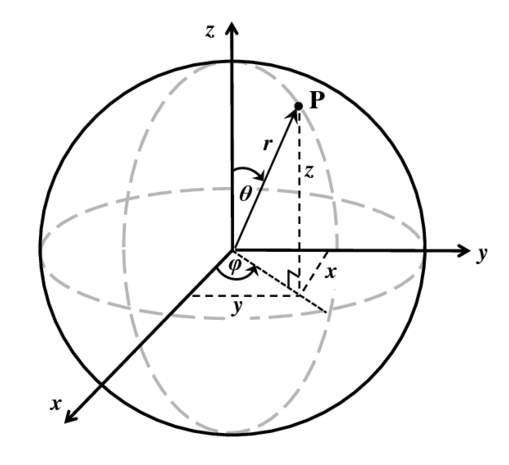
\includegraphics[width=0.45\textwidth]{../figures/lec21.2.png}
    \caption{Transforming into spherical coordinates}
    \label{fig2:21}
  \end{wrapfigure}
  For all $(x,y,z) \in \R^3 \setminus \{ (0,0,\alpha) \mid \alpha \in \R \}$, set
  \[
    (x,y,z) = (r\sin\phi\cos\theta, r\sin\phi\sin\theta, r \cos\phi)
  \]
  where $0 < \theta < 2\pi$ and $0 < \phi < \pi$. Set
  \[
    \mathcal{O}_3 := \left\{ (r,\phi,\theta) \mid r >0, \, 0 < \phi < \pi \mbox{ and } 0 < \theta < 2\pi \right\}
  \]
  and define
  \begin{align*}
    \varphi : \mathcal{O}_3 & \to \R^3, \ \varphi(r,\phi,\theta) = (x,y,z)
  \end{align*}
  Then we get
  \[
    J_{\varphi}(r,\phi,\theta) = \begin{bmatrix}
      \sin\phi\cos\theta & r\cos\phi\cos\theta & -r\sin\phi\sin\theta \\
      \sin\phi\sin\theta & r\cos\phi\sin\theta & r\sin\phi\cos\theta  \\
      \cos\phi           & -r\sin\phi          & 0
    \end{bmatrix}
  \]


  And hence $\det(J_{\varphi}(r,\phi,\theta)) = r^2 \sin \phi$, thus in the given domain $\det(J_{\varphi}(r,\phi,\theta)) \neq 0$, and hence since $\varphi$ is injective and $C^1$ function, we can use Theorem \ref{th:21:1} to transform from Cartesian to spherical coordinates. For clarity let's look at an application of spherical coordinates.

  \

  Consider $\Omega = \{ (x,y,z) \mid x^2 + y^2 + z^2 \leq a^2 \}$, then
  \begin{align*}
    \mathrm{Vol}(\Omega) & = \int_0^{2\pi}\int_0^{\pi} \int_0^a r^2 \sin \phi \, \dd r \, \dd \phi \, \dd \theta \\
                         & = \frac{4}{3}\pi a^3
  \end{align*}
\end{Eg}

\end{document}